% Options for packages loaded elsewhere
\PassOptionsToPackage{unicode}{hyperref}
\PassOptionsToPackage{hyphens}{url}
%
\documentclass[
]{article}
\usepackage{amsmath,amssymb}
\usepackage{lmodern}
\usepackage{ifxetex,ifluatex}
\ifnum 0\ifxetex 1\fi\ifluatex 1\fi=0 % if pdftex
  \usepackage[T1]{fontenc}
  \usepackage[utf8]{inputenc}
  \usepackage{textcomp} % provide euro and other symbols
\else % if luatex or xetex
  \usepackage{unicode-math}
  \defaultfontfeatures{Scale=MatchLowercase}
  \defaultfontfeatures[\rmfamily]{Ligatures=TeX,Scale=1}
\fi
% Use upquote if available, for straight quotes in verbatim environments
\IfFileExists{upquote.sty}{\usepackage{upquote}}{}
\IfFileExists{microtype.sty}{% use microtype if available
  \usepackage[]{microtype}
  \UseMicrotypeSet[protrusion]{basicmath} % disable protrusion for tt fonts
}{}
\makeatletter
\@ifundefined{KOMAClassName}{% if non-KOMA class
  \IfFileExists{parskip.sty}{%
    \usepackage{parskip}
  }{% else
    \setlength{\parindent}{0pt}
    \setlength{\parskip}{6pt plus 2pt minus 1pt}}
}{% if KOMA class
  \KOMAoptions{parskip=half}}
\makeatother
\usepackage{xcolor}
\IfFileExists{xurl.sty}{\usepackage{xurl}}{} % add URL line breaks if available
\IfFileExists{bookmark.sty}{\usepackage{bookmark}}{\usepackage{hyperref}}
\hypersetup{
  pdftitle={Explainable artificial intelligence model to predict mortality in patients presenting with acute coronary syndromes},
  hidelinks,
  pdfcreator={LaTeX via pandoc}}
\urlstyle{same} % disable monospaced font for URLs
\usepackage[margin=1in]{geometry}
\usepackage{color}
\usepackage{fancyvrb}
\newcommand{\VerbBar}{|}
\newcommand{\VERB}{\Verb[commandchars=\\\{\}]}
\DefineVerbatimEnvironment{Highlighting}{Verbatim}{commandchars=\\\{\}}
% Add ',fontsize=\small' for more characters per line
\usepackage{framed}
\definecolor{shadecolor}{RGB}{248,248,248}
\newenvironment{Shaded}{\begin{snugshade}}{\end{snugshade}}
\newcommand{\AlertTok}[1]{\textcolor[rgb]{0.94,0.16,0.16}{#1}}
\newcommand{\AnnotationTok}[1]{\textcolor[rgb]{0.56,0.35,0.01}{\textbf{\textit{#1}}}}
\newcommand{\AttributeTok}[1]{\textcolor[rgb]{0.77,0.63,0.00}{#1}}
\newcommand{\BaseNTok}[1]{\textcolor[rgb]{0.00,0.00,0.81}{#1}}
\newcommand{\BuiltInTok}[1]{#1}
\newcommand{\CharTok}[1]{\textcolor[rgb]{0.31,0.60,0.02}{#1}}
\newcommand{\CommentTok}[1]{\textcolor[rgb]{0.56,0.35,0.01}{\textit{#1}}}
\newcommand{\CommentVarTok}[1]{\textcolor[rgb]{0.56,0.35,0.01}{\textbf{\textit{#1}}}}
\newcommand{\ConstantTok}[1]{\textcolor[rgb]{0.00,0.00,0.00}{#1}}
\newcommand{\ControlFlowTok}[1]{\textcolor[rgb]{0.13,0.29,0.53}{\textbf{#1}}}
\newcommand{\DataTypeTok}[1]{\textcolor[rgb]{0.13,0.29,0.53}{#1}}
\newcommand{\DecValTok}[1]{\textcolor[rgb]{0.00,0.00,0.81}{#1}}
\newcommand{\DocumentationTok}[1]{\textcolor[rgb]{0.56,0.35,0.01}{\textbf{\textit{#1}}}}
\newcommand{\ErrorTok}[1]{\textcolor[rgb]{0.64,0.00,0.00}{\textbf{#1}}}
\newcommand{\ExtensionTok}[1]{#1}
\newcommand{\FloatTok}[1]{\textcolor[rgb]{0.00,0.00,0.81}{#1}}
\newcommand{\FunctionTok}[1]{\textcolor[rgb]{0.00,0.00,0.00}{#1}}
\newcommand{\ImportTok}[1]{#1}
\newcommand{\InformationTok}[1]{\textcolor[rgb]{0.56,0.35,0.01}{\textbf{\textit{#1}}}}
\newcommand{\KeywordTok}[1]{\textcolor[rgb]{0.13,0.29,0.53}{\textbf{#1}}}
\newcommand{\NormalTok}[1]{#1}
\newcommand{\OperatorTok}[1]{\textcolor[rgb]{0.81,0.36,0.00}{\textbf{#1}}}
\newcommand{\OtherTok}[1]{\textcolor[rgb]{0.56,0.35,0.01}{#1}}
\newcommand{\PreprocessorTok}[1]{\textcolor[rgb]{0.56,0.35,0.01}{\textit{#1}}}
\newcommand{\RegionMarkerTok}[1]{#1}
\newcommand{\SpecialCharTok}[1]{\textcolor[rgb]{0.00,0.00,0.00}{#1}}
\newcommand{\SpecialStringTok}[1]{\textcolor[rgb]{0.31,0.60,0.02}{#1}}
\newcommand{\StringTok}[1]{\textcolor[rgb]{0.31,0.60,0.02}{#1}}
\newcommand{\VariableTok}[1]{\textcolor[rgb]{0.00,0.00,0.00}{#1}}
\newcommand{\VerbatimStringTok}[1]{\textcolor[rgb]{0.31,0.60,0.02}{#1}}
\newcommand{\WarningTok}[1]{\textcolor[rgb]{0.56,0.35,0.01}{\textbf{\textit{#1}}}}
\usepackage{longtable,booktabs,array}
\usepackage{calc} % for calculating minipage widths
% Correct order of tables after \paragraph or \subparagraph
\usepackage{etoolbox}
\makeatletter
\patchcmd\longtable{\par}{\if@noskipsec\mbox{}\fi\par}{}{}
\makeatother
% Allow footnotes in longtable head/foot
\IfFileExists{footnotehyper.sty}{\usepackage{footnotehyper}}{\usepackage{footnote}}
\makesavenoteenv{longtable}
\usepackage{graphicx}
\makeatletter
\def\maxwidth{\ifdim\Gin@nat@width>\linewidth\linewidth\else\Gin@nat@width\fi}
\def\maxheight{\ifdim\Gin@nat@height>\textheight\textheight\else\Gin@nat@height\fi}
\makeatother
% Scale images if necessary, so that they will not overflow the page
% margins by default, and it is still possible to overwrite the defaults
% using explicit options in \includegraphics[width, height, ...]{}
\setkeys{Gin}{width=\maxwidth,height=\maxheight,keepaspectratio}
% Set default figure placement to htbp
\makeatletter
\def\fps@figure{htbp}
\makeatother
\setlength{\emergencystretch}{3em} % prevent overfull lines
\providecommand{\tightlist}{%
  \setlength{\itemsep}{0pt}\setlength{\parskip}{0pt}}
\setcounter{secnumdepth}{-\maxdimen} % remove section numbering
\usepackage{tikz}
\usepackage{pgfplots}
\usepackage{booktabs}
\usepackage{longtable}
\usepackage{array}
\usepackage{multirow}
\usepackage{wrapfig}
\usepackage{float}
\usepackage{colortbl}
\usepackage{pdflscape}
\usepackage{tabu}
\usepackage{threeparttable}
\usepackage{threeparttablex}
\usepackage[normalem]{ulem}
\usepackage{makecell}
\usepackage{xcolor}
\ifluatex
  \usepackage{selnolig}  % disable illegal ligatures
\fi
\newlength{\cslhangindent}
\setlength{\cslhangindent}{1.5em}
\newlength{\csllabelwidth}
\setlength{\csllabelwidth}{3em}
\newenvironment{CSLReferences}[2] % #1 hanging-ident, #2 entry spacing
 {% don't indent paragraphs
  \setlength{\parindent}{0pt}
  % turn on hanging indent if param 1 is 1
  \ifodd #1 \everypar{\setlength{\hangindent}{\cslhangindent}}\ignorespaces\fi
  % set entry spacing
  \ifnum #2 > 0
  \setlength{\parskip}{#2\baselineskip}
  \fi
 }%
 {}
\usepackage{calc}
\newcommand{\CSLBlock}[1]{#1\hfill\break}
\newcommand{\CSLLeftMargin}[1]{\parbox[t]{\csllabelwidth}{#1}}
\newcommand{\CSLRightInline}[1]{\parbox[t]{\linewidth - \csllabelwidth}{#1}\break}
\newcommand{\CSLIndent}[1]{\hspace{\cslhangindent}#1}

\title{Explainable artificial intelligence model to predict mortality in
patients presenting with acute coronary syndromes}
\usepackage{etoolbox}
\makeatletter
\providecommand{\subtitle}[1]{% add subtitle to \maketitle
  \apptocmd{\@title}{\par {\large #1 \par}}{}{}
}
\makeatother
\subtitle{Edwin Kagereki - B00867154}
\author{}
\date{\vspace{-2.5em}13 November 2021}

\begin{document}
\maketitle

{
\setcounter{tocdepth}{2}
\tableofcontents
}
\hypertarget{business-understanding}{%
\section{Business Understanding}\label{business-understanding}}

\hypertarget{introduction}{%
\subsection{Introduction}\label{introduction}}

Cardiovascular diseases (CVDs), principally ischemic heart disease (IHD)
and cardiac stroke, are the leading cause of mortality globally and are
often associated with poor survival(Roth 2020).

Acute Coronary Syndrome (ACS) is a term given to diverse presentations
related to cardic myopathies of quick onset. Accurate estimation of risk
for untoward outcomes after a suspected onset of an ACS may help
clinicians chose the type and intensity of therapy. For example,
patients predicted to be at higher risk may receive more aggressive
surveillance and/or treatment, while patients predicted to be at lower
risk may be managed less aggressively.

\hypertarget{problem-statement}{%
\paragraph{Problem statement}\label{problem-statement}}

The establishment of prognosis model for patients with suspected ACS is
important in critical care medicine.Numerous risk-prediction models for
differing outcomes exist for the different types of ACS.

These models however have some limitations. First, most models have been
developed from large randomized clinical trial populations in which the
generalizability to risk prediction in the average clinician's
experience is questionable(Eagle KA Lim MJ 2004).Second, given the
dynamic nature of the treatment environment, predicting future behavior
while the treatment is underway may help the clinicians make decisions
proactively.

This project aimed at developing a risk-prediction tool for ACS,
focusing on clinical end point of all-cause mortality using multiple
linked ICU patients' datasets. Subsequently, the treatment pathway was
used to explain the predicted outcome.

\hypertarget{project-objectives}{%
\subsubsection{Project Objectives}\label{project-objectives}}

This project developed a tool for application in the decision-making
environment. This was done in two steps:

\begin{enumerate}
\def\labelenumi{\arabic{enumi}.}
\tightlist
\item
  A binary classification model was developed. This model used:
\end{enumerate}

\begin{itemize}
\tightlist
\item
  Patient demographics
\item
  Interventions within the golden hour (laboratory, medication,
  procedures and microbiology studies).Although not set in stone, the
  chances for a patient to have good outcomes are usually high if
  substantive medical attention is given within an hour of the cardiac
  event(Johnson 2016). In this study the golden hour cut-off was 60
  minutes after initial contact with the hospital. This included all
  interventions that were done prior to admission.
\end{itemize}

\begin{enumerate}
\def\labelenumi{\arabic{enumi}.}
\setcounter{enumi}{1}
\tightlist
\item
  Process mining was used to explain the outcome of the patient based on
  the care pathway followed. Two concepts were applied:
\end{enumerate}

\begin{itemize}
\tightlist
\item
  Process discovery - Processes followed by the two classes will be
  described.
\item
  Conformance checking - The care pathway followed by both patients will
  be checked for conformance with the American Heart Association(AHA)
  guidelines for CPR and ECC (ACLS 2020). To run the process mining the
  timestamped interventions (laboratory, medication, procedures) were
  used.
\end{itemize}

\hypertarget{project-plan}{%
\subsection{Project plan}\label{project-plan}}

\hypertarget{sources-of-data-and-knowledge}{%
\paragraph{Sources of Data and
Knowledge}\label{sources-of-data-and-knowledge}}

\hypertarget{mimic-iii-database}{%
\subparagraph{MIMIC III Database}\label{mimic-iii-database}}

MIMIC-III is a large, freely-available database comprising deidentified
health-related data associated with 46,520 patients who stayed in
critical care units of the Beth Israel Deaconess Medical Center between
2001 and 2012. The database includes information such as demographics,
vital sign measurements made at the bedside , laboratory test results,
procedures, medications, caregiver notes, imaging reports, and mortality
(including post-hospital discharge).

Although de-identified, the datasets described herein contain detailed
information regarding the clinical care of patients, and as such it must
be treated with appropriate care and respect.

Researchers seeking to use the database must:

\begin{enumerate}
\def\labelenumi{\arabic{enumi}.}
\tightlist
\item
  Become a credentialed user on
  \href{https://physionet.org/}{PhysioNet.} This involves completion of
  a training course in human subjects research.
\item
  Sign the data use agreement. Adherence to the terms of the DUA is
  paramount.
\end{enumerate}

\hypertarget{loic-tables}{%
\subparagraph{LOIC tables}\label{loic-tables}}

The Loin(Institute 2021) data tables will be used to enrich the
laboratory dataset.

\hypertarget{american-heart-association-guidelines-for-cpr-and-ecc}{%
\subparagraph{American Heart Association guidelines for CPR and
ECC}\label{american-heart-association-guidelines-for-cpr-and-ecc}}

This AHA guideline(ACLS 2020) will be used as the gold standard for ACS
workflow. The workflows for the patients in this project will be
assessed for cornformity with this workflow.

\hypertarget{terminology}{%
\subsubsection{Terminology}\label{terminology}}

\begin{enumerate}
\def\labelenumi{\arabic{enumi}.}
\tightlist
\item
  \textbf{Acute Cardiac syndrome:} Acute coronary syndrome (ACS) refers
  to a spectrum of clinical presentations ranging from those for
  ST-segment elevation myocardial infarction (STEMI) to presentations
  found in non--ST-segment elevation myocardial infarction (NSTEMI) or
  in unstable angina. It is almost always associated with rupture of an
  atherosclerotic plaque and partial or complete thrombosis of the
  infarct-related artery. Candidates of acute cardiac syndrome were
  identified using the \emph{DIAGNOSIS} in the \emph{ADMISSIONS} table
  which provides a preliminary. This column was is a free text diagnosis
  for the patient on hospital admission. The diagnosis was assigned by
  the admitting clinician and did use a systematic ontology. Candidate
  cased were identified by using the key words commonly used in the
  diagnosis of acute coronary syndrome and the related differential
  diagnosis. These were:
\end{enumerate}

\emph{``stemi,''``acute coronary
syndrome,''``angina,''``tachycardia,''``aortic
aneurysm,''``pericardi,''``ortic dissection,''``coronary artery
dissection,''``cardiomyopathy,''``heart failure,''``mitral valve
disease,''``mitral stenosis,''``coronary artery
disease,''``chf,''``congestive heart failure,''``heart
failure,''``telemetry,''``myocardial infaction,''``cardiac
arrest,''``myocardial infarction,''``aortic stenosis,''``st
elevated,''``pericardial effusion,'' ``cardiomyopathy,''``cath
lab,''``tamponade,''``tamponede''}

\begin{enumerate}
\def\labelenumi{\arabic{enumi}.}
\setcounter{enumi}{1}
\tightlist
\item
  Angiotensin-converting enzyme (ACE) inhibitors are medications that
  help relax the veins and arteries to lower blood pressure. ACE
  inhibitors prevent an enzyme in the body from producing angiotensin
  II, a substance that narrows blood vessels. The following terms were
  used to identify ACE's from the list of \emph{DRUG} column of the
  \emph{PRESCRIPTIONS TABLE} table:
\end{enumerate}

\emph{``benazepril,'' ``captopril,''
``enalapril,''``enalaprilat,''``fosinopril,'' ``lisinopril,''
``moexipril,'' ``perindopril,'' ``quinapril,''
``ramipril,''``trandolapril''}

\begin{enumerate}
\def\labelenumi{\arabic{enumi}.}
\setcounter{enumi}{2}
\tightlist
\item
  Beta blockers (beta-adrenergic blocking agents)
\end{enumerate}

Medications that reduce blood pressure. Beta blockers work by blocking
the effects of the hormone epinephrine, also known as adrenaline.The
following terms were used to identify Beta blocker from the list of
\emph{DRUG} column of the \emph{PRESCRIPTIONS TABLE} table:

\emph{``acebutolol,''``atenolol,''``betaxolol,''``bisoprolol,''``carteolol,''``carvedilol,''``labetalol,''``metoprolol,''``nadolol,''``nebivolol,''}
\emph{``penbutolol,''``pindolol,''``propanolol,''``sotalol,''``timolol''}

\begin{enumerate}
\def\labelenumi{\arabic{enumi}.}
\setcounter{enumi}{3}
\tightlist
\item
  Glycoprotein IIb/IIIa inhibitors
\end{enumerate}

These drugs are frequently used during percutaneous coronary
intervention (angioplasty with or without intracoronary stent
placement). They work by preventing platelet aggregation and thrombus
formation.

The following terms were used to identify Glycoprotein IIb/IIIa
inhibitors's from the list of \emph{DRUG} column of the
\emph{PRESCRIPTIONS TABLE} table:

\emph{``abciximab,''``eptifibatide,''``tirofiban,''``roxifiban,''``orbofiban''}

\begin{enumerate}
\def\labelenumi{\arabic{enumi}.}
\setcounter{enumi}{4}
\item
  P2Y12 inhibitors
  \emph{``clopidogrel,''``prasugrel,''``ticlopidine,''``ticagrelor''}
\item
  HMGCoA
  \emph{``altoprev,''``amlodipine,''``atorvastatin,''``caduet,''``crestor,''``ezallor,''``fluvastatin,''``lescol,''``lipitor,''``livalo,''``lovastatin,''``mevacor,''``pitavastatin,''``pravachol,''``pravastatin,''``rosuvastatin,''``simcor,''``simvastatin,''``simvastatin,''``ezetimibe,''``simvastatin,''``niacin,''``vytorin,''``zocor,''``zypitamag''}
\item
  A glossary of data mining terminology, illustrated with examples
  relevant to the business problem in question
\end{enumerate}

\begin{itemize}
\tightlist
\item
  Check prior availability of glossaries; otherwise begin to draft
  glossaries
\item
  Talk to domain experts to understand their terminology
\item
  Become familiar with the business terminology
\end{itemize}

\hypertarget{inventory-of-resources}{%
\subsubsection{Inventory of resources}\label{inventory-of-resources}}

\hypertarget{software}{%
\paragraph{Software}\label{software}}

For this project the following software will be used:

\begin{enumerate}
\def\labelenumi{\arabic{enumi}.}
\tightlist
\item
  PostgreSQL
\item
  R
\item
  Python
\end{enumerate}

\hypertarget{computing-resources}{%
\paragraph{Computing resources}\label{computing-resources}}

The analysis will be done on a Windows desktop and a Linux server.
\href{https://github.com/em-kagereki/Data-Mining}{Github repository} was
used for the CI/CD pipeline.

\hypertarget{requirements-assumptions-and-constraints}{%
\subsubsection{Requirements, Assumptions, and
Constraints}\label{requirements-assumptions-and-constraints}}

For this analysis, the all the medical records were not analysed.

It is also assumed that:

\begin{itemize}
\item
  The patients in this population were only treated in this hospital,
  therefore mortality are only captured in this hospital.
\item
  All the pre-hospitalization interventions were captured.
\end{itemize}

\hypertarget{risks-and-contingencies}{%
\subsubsection{Risks and Contingencies}\label{risks-and-contingencies}}

\begin{itemize}
\tightlist
\item
  Although the process mining will give a better predictive description
  of the patient outcomes, alternative surrogate modeling methods like
  decision tree maybe used.
\end{itemize}

\hypertarget{data-mining-goals}{%
\subsubsection{Data Mining Goals}\label{data-mining-goals}}

\begin{enumerate}
\def\labelenumi{\arabic{enumi}.}
\tightlist
\item
  Build a binary classification machine learning model to predict
  all-cause mortality of patients based on demographics and
  interventions within first hour of suspected ACS event.
\item
  Compare the conformity of care path in patients who died and patients
  who survived with the with the ACLS care path.
\item
  Assess and report any work flow variants, and differences between
  patients who died and those who survived.
\end{enumerate}

The success of this project was to generate forward-looking, predictive
insights to improve the management of the care pathway in patients
suspected to have ACS by:

\begin{itemize}
\tightlist
\item
  Successfully predicting the ICU mortality outcome of the patient with
  suspected ACS based on the patient demographics and the interventions
  given within the first one hour.
\item
  Identify patients in which undesirable events will likely be observed
  in the based on the interventions.
\end{itemize}

\hypertarget{data-mining-success-criteria}{%
\subsubsection{Data Mining Success
Criteria}\label{data-mining-success-criteria}}

After training the binary classifier, evaluation measures will be used
to assess the performance of the model. The predictive performance of
the classifier will be assessed by calculating the number of correctly
identified class patients (true positives), the number of correctly
recognized patients that are not member of the class (true negatives),
the number of the patients that are wrongly recognized (false positives)
and the number of the examples that were not identified (false
negatives). By using these measures, a confusion matrix will be
constituted.

\begin{longtable}[]{@{}clcc@{}}
\toprule
& & Ground Truth Values & \\
\midrule
\endhead
& & Positive & Negative \\
Predicted Values & Positive & true positive (tp) & false positive
(fp) \\
& Negative & false negative (fn) & true negative (tn) \\
\bottomrule
\end{longtable}

The following measures will be calculated from this table:

\begin{itemize}
\tightlist
\item
  Accuracy.
\item
  Precision.
\item
  Recall.
\item
  Specificity.
\end{itemize}

To benchmark the classification model performance, the results ranging
from accuracy of (70\% to 90\%) as reported in larger, though different
models used in the prediction of mortality in CVDs will be used(Sherazi
et al.~2020).

\hypertarget{data-understanding}{%
\section{Data Understanding}\label{data-understanding}}

\hypertarget{data-access}{%
\subsection{Data Access}\label{data-access}}

Having met the criterian and gained access, I also learned about and
calculated various severity scores for each patient which I will talk
about later on in the article. When allowed access to the MIMIC-III
database, it is suggested that you transfer all of this information into
a RDMS (relational database management system) and Physionet has
tutorials on how to transfer the database into a local instance of the
PostgreSQL RDMS which I followed. After connecting to the PostgreSQL
database, I was able to easily make SQL queries and connect my database
to many helpful tools such as pgAdmin4 which provides a GUI (graphical
user interface) for the database.

Although the database includes 26 tables, only the following tables will
be included in the analysis:

\begin{itemize}
\tightlist
\item
  \textbf{ADMISSIONS:} Contains information regarding a patient's
  admission to the hospital. Information available includes timing
  information for admission and discharge, demographic information, the
  source of the admission, and so on. Record of 58,976 unique
  admissions.
\item
  \textbf{PATIENTS:}Defines each patient in the database, i.e.~defines a
  single patient. There are 46,520 patients recorded.
\item
  \textbf{SERVICES:}Lists services that a patient was
  admitted/transferred under.This table contains 73,343 entries.
\item
  \textbf{DIAGNOSIS\_ICD}Identify type of data sources (online sources,
  experts, written documentation, etc.)
\item
  \textbf{MICROBIOLOGYEVENTS:}Contains microbiology information,
  including cultures acquired and associated sensitivities.There are
  631,726 rows in this table.
\item
  \textbf{PRESCRIPTIONS:}Contains medication related order entries,
  i.e.~prescriptions.This table contains 4,156,450 rows.
\item
  \textbf{PROCEDUREEVENTS\_MV:}Contains procedures for patients. This
  table has 258,066 rows.
\item
  \textbf{D\_ITEMS:} Definition table for all 12,487 items in the ICU
  databases.
\item
  \textbf{D\_LABITEMS:} Definition table for 753 laboratory
  measurements.
\end{itemize}

\hypertarget{selection-criteria}{%
\subsubsection{Selection criteria}\label{selection-criteria}}

For this analysis only the patients admitted with suspected acute
cardiac syndrome were included. In this subset, patients who died within
the first hour of treatment were also excluded.

\hypertarget{derived-variables-of-data}{%
\subsubsection{Derived variables of
data}\label{derived-variables-of-data}}

The following derived variables were calculated:

\begin{enumerate}
\def\labelenumi{\arabic{enumi}.}
\item
  Age - The age was computed by subtracting the \emph{DOB} from the
  \emph{ADMITTIME}. Any figure above 300 was adjusted by subtracting
  211, since any age above 300 was ages over 89 had been shifted such
  that the patient age appears to be 300 in the database.
\item
  Splitting of Datetime Features - The following features were extracted
  from teh \emph{ADMITTIME} feature:
\end{enumerate}

\begin{itemize}
\tightlist
\item
  Day of the year
\item
  Week of the year
\item
  Month
\item
  Year
\item
  Hour of day
\end{itemize}

\begin{enumerate}
\def\labelenumi{\arabic{enumi}.}
\setcounter{enumi}{2}
\item
  The Length of stay: This was calculated from the previous admissions.
\item
  Admission cycle: If the patient had multiple admissions, what was the
  admission cycle in this case.
\end{enumerate}

\hypertarget{data-exploration}{%
\subsection{Data exploration}\label{data-exploration}}

The MIMIC III dataset contained 20399 43.85 female and \% and 26121
56.15 male patients. The cumulative incidence of suspected ACS was
24.11\%. The report is summarized in Table 1 below.

These data was subset using a total of unique subset of the words as
shown below.

In addition the patients were seen over a span of time ranging from
2100-07-09 to 2209-07-14. This temporal distribution is shown in the
chart below:

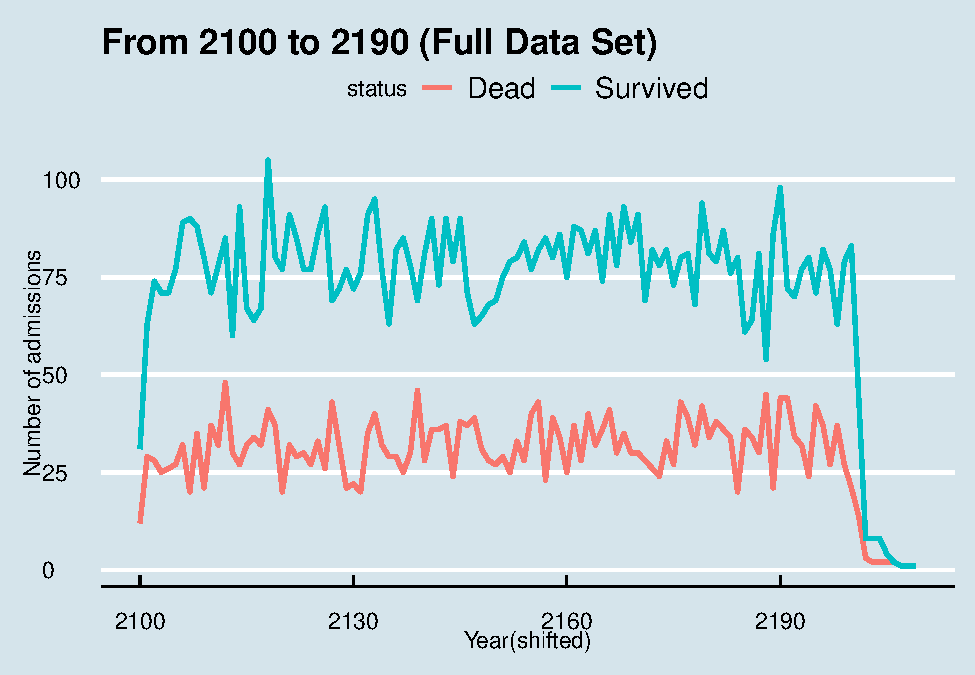
\includegraphics{MyReport_files/figure-latex/unnamed-chunk-4-1.pdf}

\hypertarget{volumetric-analysis-of-data}{%
\subsubsection{Volumetric analysis of
data}\label{volumetric-analysis-of-data}}

The total dataset was estimated to be more than 100GBs of data. The
selected subset of data tables was about 3.47 GBs.

\hypertarget{attribute-types-and-values}{%
\subsubsection{Attribute types and
values}\label{attribute-types-and-values}}

And see Table @Table 2.

\hypertarget{assumptionslimitations}{%
\subsubsection{Assumptions/Limitations}\label{assumptionslimitations}}

\begin{itemize}
\tightlist
\item
  The patients in this population were only treated in this hospital,
  therefore all important events like hospitalization and mortality are
  only captured in this hospital.
\item
  All the pre-hospitalization interventions were captured.
\item
  The unit of analysis is the admission
\end{itemize}

\hypertarget{data-preparation}{%
\section{Data Preparation}\label{data-preparation}}

Data quality was assessed dimensions of completeness, uniqueness,
validity, accuracy and consistency. Any issue picked was addressed in
the data cleaning step below.

\hypertarget{data-cleaning}{%
\subsection{Data Cleaning}\label{data-cleaning}}

\begin{enumerate}
\def\labelenumi{\arabic{enumi}.}
\tightlist
\item
  There were no duplicates.
\item
  Completeness:
\end{enumerate}

\begin{itemize}
\tightlist
\item
  Any treatment offered before admission had missing admission
  ID(\emph{ADMISSION.HADM\_ID}). This was inferred from the patient id
  (\emph{ADMISSION.SUBJECT\_ID}) and treatment period.
\item
  The language(\emph{ADMISSION.LANGUAGE}) and ethnicity
  (\emph{ADMISSION.ETHNICITY}). These were replaced with ``UNKNOWN''
\end{itemize}

\begin{enumerate}
\def\labelenumi{\arabic{enumi}.}
\setcounter{enumi}{2}
\tightlist
\item
  Consistency:
\end{enumerate}

\begin{itemize}
\tightlist
\item
  The diagnosis(\emph{ADMISSION.DIAGNOSIS}) provides a preliminary, free
  text diagnosis for the patient on hospital admission as assigned by
  the admitting clinician and does not use a systematic ontology. Data
  cleaning was done by removing unnecessary text and ensuring common
  acronyms and abbreviations referred to the same diagnosis.
\item
  The Loinc table was used to identify the actual test.
\end{itemize}

\hypertarget{categorical-variable-encoding}{%
\subsection{Categorical variable
encoding}\label{categorical-variable-encoding}}

\begin{enumerate}
\def\labelenumi{\arabic{enumi}.}
\tightlist
\item
  Categorical variables with high cardinality: diagnoses, medicine,
  procedures.
\end{enumerate}

\begin{itemize}
\tightlist
\item
  This target encoding/hash encoding was used.
\end{itemize}

\begin{enumerate}
\def\labelenumi{\arabic{enumi}.}
\setcounter{enumi}{1}
\tightlist
\item
  Categorical variables with less cardinality but need to preserve the
  variance: gender,
\end{enumerate}

\begin{itemize}
\tightlist
\item
  Frequency encoding was used
\end{itemize}

\hypertarget{dimension-reduction}{%
\subsection{Dimension reduction}\label{dimension-reduction}}

Principal componet analysis was used to reduce the dimensionality of the
data.

\url{https://towardsdatascience.com/dimensionality-reduction-for-data-visualization-pca-vs-tsne-vs-umap-be4aa7b1cb29}

\hypertarget{final-dataset}{%
\subsection{Final Dataset}\label{final-dataset}}

Finally the chosen dataset factoring in 90\% of the variance was
factored in. This was used for the final analysis.

\hypertarget{construction-of-event-logs}{%
\subsection{Construction of event
logs}\label{construction-of-event-logs}}

\hypertarget{modeling}{%
\section{Modeling}\label{modeling}}

\hypertarget{data-splitting}{%
\subsection{Data splitting}\label{data-splitting}}

For the data splitting strategy, 25\% of the hospital admissions were
reserved to the test set.

The k-fold cross-validation resampling method was used to create 5
different resamples of the training set which were further split into
analysis and assessment sets, producing 5 different performance metrics
that were then aggregated. In these resampled datasets, 20\% of the
hospital admissions were allocated to the validation set and 80\% of the
hospital stays to the training set.

\begin{tikzpicture}[sibling distance=10em,
  every node/.style = {shape=rectangle, rounded corners,
    draw, align=center,
    top color=white, bottom color=blue!20}]]
  \node {All data= 11215}
      child { node {Testing $\sim$2804} }
      child { node {Training $\sim$ 8411}
      child { node {Sample 1 $\sim$ 1682}
      child { node {Training $\sim$1346}} 
      child { node {Validation $\sim$336} }}
      child { node {.....}}
      child { node {Sample 5 $\sim$ 1682}
      child { node {Training $\sim$1346}} 
      child { node {Validation $\sim$336} }}};
\caption{M1} \label{fig:M1}

\end{tikzpicture}

\hypertarget{model-building-and-tuning}{%
\subsection{Model building and tuning}\label{model-building-and-tuning}}

\hypertarget{performance-metric-and-cut-off-analysis}{%
\subsubsection{Performance metric and cut-off
analysis}\label{performance-metric-and-cut-off-analysis}}

In this analysis the F-Beta score was used to identify the model with
the highest performance with a score 1.This was meant to:

Increase Precision is a metric that calculates the percentage of correct
predictions for the positive class.

Recall calculates the percentage of correct predictions for the positive
class out of all positive predictions that could be made.

The selected Beta score of 1 was meant to maximize precision will
minimize the false-positive errors, whereas maximizing recall will
minimize the false-negative errors.

Finally all the performance metrics of this model were described.

\hypertarget{candidate-models}{%
\paragraph{Candidate models}\label{candidate-models}}

The following candidate models will first be assessed.

\begin{itemize}
\tightlist
\item
  Logistic Regression
\item
  Random Forest,
\item
  XGBoost (extreme gradient boosted trees),
\item
  K-nearest neighbor
\end{itemize}

\hypertarget{model-building-and-tuning-1}{%
\paragraph{Model building and
tuning}\label{model-building-and-tuning-1}}

Grid search algorithm was used to train multiple models simultaneously.
We'll also save the validation set predictions (via the call to
control\_grid()) so that diagnostic information can be available after
the model fit. The area under the ROC curve will be used to quantify how
well the model performs across a continuum of event thresholds (recall
that the event rate---the proportion of stays including children--- is
very low for these data).

We will use a space-filling design to tune, with 25 candidate models:
The random forest is uniformly better across event probability
thresholds.

The combination that provides the best performance is the one that you
use for your final model. This method is simple to use. You can find the
best combination of the values that you provided, and you can run each
of the experiments in parallel. However, it's also computationally
expensive because so many models are being built. If a hyperparameter
isn't important, you might explore different possibilities
unnecessarily.

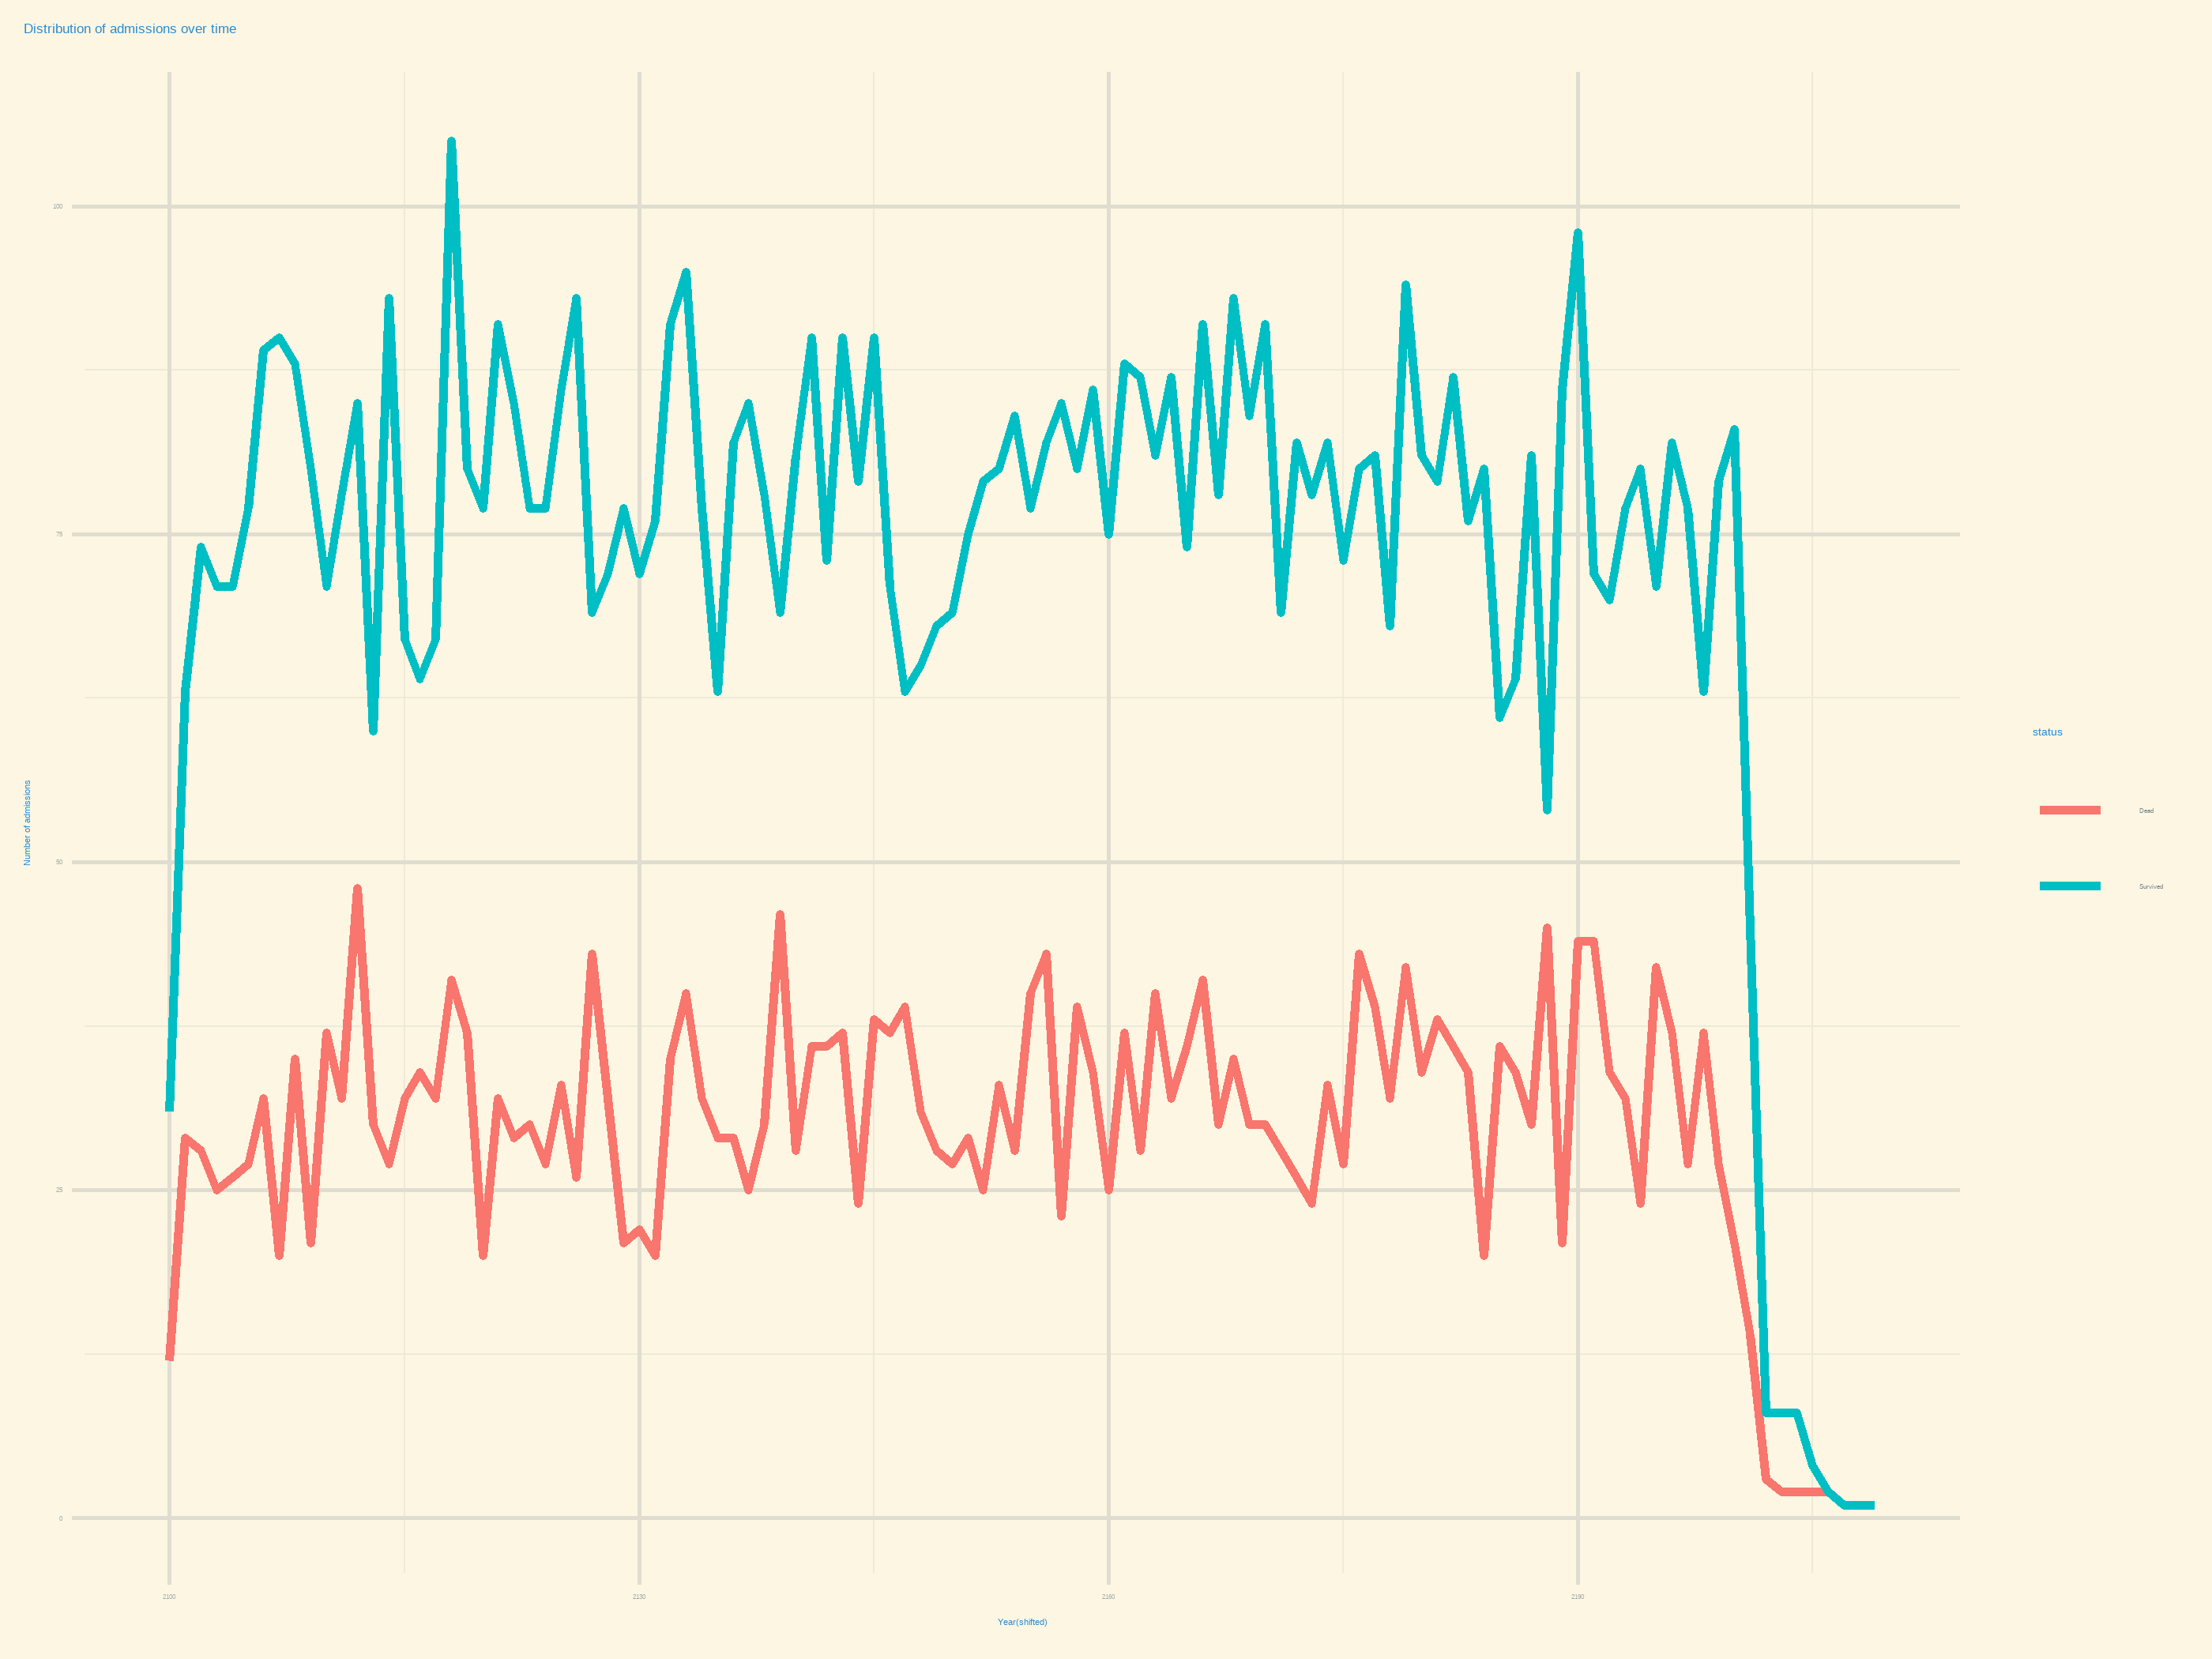
\includegraphics{MyReport_files/figure-latex/unnamed-chunk-6-1.pdf}
\includegraphics{MyReport_files/figure-latex/unnamed-chunk-6-2.pdf}

\hypertarget{best-model-description}{%
\subsubsection{Best model Description}\label{best-model-description}}

\hypertarget{deployment}{%
\section{Deployment}\label{deployment}}

\hypertarget{plan-deployment}{%
\subsection{Plan Deployment}\label{plan-deployment}}

This task starts with the evaluation results and concludes with a
strategy for deployment of the data mining result(s) into the business.

\hypertarget{deployment-plan}{%
\subsubsection{Deployment Plan}\label{deployment-plan}}

Summarize the deployment strategy, including necessary steps and how to
perform them.

\begin{itemize}
\tightlist
\item
  Summarize deployable results
\item
  Develop and evaluate alternative plans for deployment
\item
  Decide for each distinct knowledge or information result
\item
  Determine how knowledge or information will be propagated to users
\item
  Decide how the use of the result will be monitored and its benefits
  measured (where applicable)
\item
  Decide for each deployable model or software result
\item
  Establish how the model or software result will be deployed within the
  organization's systems
\item
  Determine how its use will be monitored and its benefits measured
  (where applicable)
\item
  Identify possible problems during deployment (pitfalls to be avoided)
\end{itemize}

\hypertarget{plan-monitoring-and-maintenance}{%
\subsection{Plan Monitoring and
Maintenance}\label{plan-monitoring-and-maintenance}}

Monitoring and maintenance are important issues if the data mining
results become part of the day-to-day business and its environment. A
careful preparation of a maintenance strategy helps to avoid
unnecessarily long periods of incorrect usage of data mining results. In
order to monitor the deployment of the data mining result(s), the
project needs a detailed plan for monitoring and maintenance. This plan
takes into account the specific type of deployment.

\hypertarget{monitoring-and-maintenance-plan}{%
\subsubsection{Monitoring and Maintenance
Plan}\label{monitoring-and-maintenance-plan}}

Summarize monitoring and maintenance strategy, including necessary steps
and how to perform them.

\begin{itemize}
\tightlist
\item
  Check for dynamic aspects (i.e., what things could change in the
  environment?)
\item
  Decide how accuracy will be monitored
\item
  Determine when the data mining result or model should not be used any
  more. Identify criteria (validity, threshold of accuracy, new data,
  change in the application domain, etc.), and what should happen if the
  model or result could no longer be used. (update model, set up new
  data mining project, etc.).
\item
  Will the business objectives of the use of the model change over time?
  Fully document the initial problem the model was attempting to solve.
\item
  Develop monitoring and maintenance plan.
\end{itemize}

\hypertarget{produce-final-report}{%
\subsection{Produce Final Report}\label{produce-final-report}}

At the end of the project, the project team writes up a final report.
Depending on the deployment plan, this report may be only a summary of
the project and its experience, or a final presentation of the data
mining result(s).

\hypertarget{final-report}{%
\subsubsection{Final Report}\label{final-report}}

At the end of the project, there will be at least one final report in
which all the threads are brought together. As well as identifying the
results obtained, the report should also describe the process, show
which costs have been incurred, define any deviations from the original
plan, describe implementation plans, and make any recommendations for
future work. The actual detailed content of the report depends very much
on the intended audience.

\begin{itemize}
\tightlist
\item
  Identify what reports are needed (slide presentation, management
  summary, detailed findings, explanation of models, etc.)
\item
  Analyze how well initial data mining goals have been met
\item
  Identify target groups for report
\item
  Outline structure and contents of report(s)
\item
  Select findings to be included in the reports
\item
  Write a report
\end{itemize}

\hypertarget{final-presentation}{%
\subsubsection{Final Presentation}\label{final-presentation}}

As well as a final report, it may be necessary to make a final
presentation to summarize the project -- maybe to the management
sponsor, for example. The presentation normally contains a subset of the
information contained in the final report, structured in a different
way.

\begin{itemize}
\tightlist
\item
  Decide on target group for the final presentation and determine if
  they will already have received the final report
\item
  Select which items from the final report should be included in final
  presentation
\end{itemize}

\hypertarget{review-project}{%
\subsection{Review Project}\label{review-project}}

Assess what went right and what went wrong, what was done well, and what
needs to be improved.

\hypertarget{experience-documentation}{%
\subsubsection{Experience
Documentation}\label{experience-documentation}}

Summarize important experience gained during the project. For example,
pitfalls, misleading approaches, or tips for selecting the best-suited
data mining techniques in similar situations could be part of this
documentation. In ideal projects, experience documentation also covers
any reports that have been written by individual project members during
the project.

\begin{itemize}
\tightlist
\item
  Interview all significant people involved in the project and ask them
  about their experience during the project
\item
  If end users in the business work with the data mining result(s),
  interview them: Are they satisfied? What could have been done better?
  Do they need additional support?
\item
  Summarize feedback and write the experience documentation
\item
  Analyze the process (things that worked well, mistakes made, lessons
  learned, etc.)
\item
  Document the specific data mining process (How can the results and the
  experience of applying the model be fed back into the process?)
\item
  Generalize from the details to make the experience useful for future
  projects
\end{itemize}

\hypertarget{appendix}{%
\section{Appendix}\label{appendix}}

\begin{Shaded}
\begin{Highlighting}[]
\NormalTok{con }\OtherTok{\textless{}{-}}\NormalTok{ DBI}\SpecialCharTok{::}\FunctionTok{dbConnect}\NormalTok{(RPostgreSQL}\SpecialCharTok{::}\FunctionTok{PostgreSQL}\NormalTok{(), }
  \AttributeTok{host =} \StringTok{"AWS end point"}\NormalTok{,}
  \AttributeTok{user =} \StringTok{"eKagereki"}\NormalTok{,}
  \AttributeTok{password =}\NormalTok{ rstudioapi}\SpecialCharTok{::}\FunctionTok{askForPassword}\NormalTok{(}\StringTok{"Database password"}\NormalTok{)}
\NormalTok{)}

\NormalTok{data }\OtherTok{\textless{}{-}} \FunctionTok{tbl}\NormalTok{(con, }\StringTok{"ADMISSIONS"}\NormalTok{)}
\end{Highlighting}
\end{Shaded}

\hypertarget{data-attibutes-and-levels-of-measurements}{%
\subsubsection{Data attibutes and levels of
measurements}\label{data-attibutes-and-levels-of-measurements}}

\begin{table}

\caption{\label{tab:dtypes}Attributes and the level of measurement}
\centering
\begin{tabular}[t]{l|l|l|r|r|r}
\hline
  & variables & types & missing\_percent & unique\_count & unique\_rate\\
\hline
7 & AGE & integer & 0 & 84 & 0.0074900\\
\hline
10 & admissionCycle & integer & 0 & 26 & 0.0023183\\
\hline
12 & deadBefore & numeric & 0 & 926 & 0.0825680\\
\hline
13 & dayOfYear & integer & 0 & 366 & 0.0326349\\
\hline
14 & Month & integer & 0 & 12 & 0.0010700\\
\hline
15 & week & integer & 0 & 53 & 0.0047258\\
\hline
16 & weekday & integer & 0 & 7 & 0.0006242\\
\hline
17 & year & integer & 0 & 110 & 0.0098083\\
\hline
18 & hour & integer & 0 & 24 & 0.0021400\\
\hline
19 & FreqGENDER & numeric & 0 & 2 & 0.0001783\\
\hline
20 & FreqADMISSION\_TYPE & numeric & 0 & 3 & 0.0002675\\
\hline
21 & FreqADMISSION\_LOCATION & numeric & 0 & 6 & 0.0005350\\
\hline
22 & FreqINSURANCE & numeric & 0 & 5 & 0.0004458\\
\hline
23 & FreqRELIGION & numeric & 0 & 20 & 0.0017833\\
\hline
24 & FreqMARITAL\_STATUS & numeric & 0 & 8 & 0.0007133\\
\hline
25 & FreqETHNICITY & numeric & 0 & 26 & 0.0023183\\
\hline
27 & FreqLANGUAGE & numeric & 0 & 23 & 0.0020508\\
\hline
\end{tabular}
\end{table}

\hypertarget{references}{%
\section*{References}\label{references}}
\addcontentsline{toc}{section}{References}

\hypertarget{refs}{}
\begin{CSLReferences}{1}{0}
\leavevmode\hypertarget{ref-americanheart}{}%
ACLS. 2020. {``Acute Coronary Syndromes Algorithm - ACLS Version
Control: This Document Follows 2020 American Heart Association
Guidelines for CPR and ECC. American Heart Association Guidelines Are
Updated Every Five Years.''}
\url{https://www.acls.net/images/algo-acs.pdf}.

\leavevmode\hypertarget{ref-Eagle}{}%
Eagle KA Lim MJ, et al., Dabbous OH. 2004. {``A Validated Prediction
Model for All Forms of Acute Coronary Syndrome: Estimating the Risk of
6-Month Postdischarge Death in an International Registry.''}
\emph{Jama}. \url{https://doi.org/doi:10.1001/jama.291.22.2727}.

\leavevmode\hypertarget{ref-loinc}{}%
Institute, Regenstrief. 2021. {``LOINC.''} \emph{LOINC}.
\url{https://loinc.org/downloads/}.

\leavevmode\hypertarget{ref-johnson}{}%
Johnson, et al, A. 2016. {``{MIMIC}-{III} {Clinical} {Database}.''}
https://doi.org/\url{https://doi.org/10.13026/C2XW26}.

\leavevmode\hypertarget{ref-roth}{}%
Roth, et al, Gregory A. 2020. {``Global Burden of Cardiovascular
Diseases and Risk Factors, 1990-2019: Update from the GBD 2019 Study.''}
\emph{Journal of the American College of Cardiology} 76 (25):
2982--3021. \url{https://doi.org/10.1016/j.jacc.2020.11.010}.

\end{CSLReferences}

\end{document}
